\documentclass[]{report}
\usepackage[german]{babel}    % Deutsche Sprache in automatisch generiertem
\usepackage{lmodern}
\usepackage{amssymb,amsmath}
\usepackage{ifxetex,ifluatex}
\usepackage{fixltx2e} % provides \textsubscript
\ifnum 0\ifxetex 1\fi\ifluatex 1\fi=0 % if pdftex
  \usepackage[T1]{fontenc}
  \usepackage[utf8]{inputenc}
\else % if luatex or xelatex
  \ifxetex
    \usepackage{mathspec}
  \else
    \usepackage{fontspec}
  \fi
  \defaultfontfeatures{Ligatures=TeX,Scale=MatchLowercase}
\fi
% use upquote if available, for straight quotes in verbatim environments
\IfFileExists{upquote.sty}{\usepackage{upquote}}{}
% use microtype if available
\IfFileExists{microtype.sty}{%
\usepackage[]{microtype}
\UseMicrotypeSet[protrusion]{basicmath} % disable protrusion for tt fonts
}{}
\PassOptionsToPackage{hyphens}{url} % url is loaded by hyperref
\usepackage[
	unicode=true,
	colorlinks=true,
	urlcolor=blue,
	linkcolor=black
]{hyperref}
\hypersetup{
            pdftitle={arc42 Template},
            pdfborder={0 0 0},
            breaklinks=true}
\urlstyle{same}  % don't use monospace font for urls
\usepackage{longtable,booktabs}
% Fix footnotes in tables (requires footnote package)
\IfFileExists{footnote.sty}{\usepackage{footnote}\makesavenoteenv{long table}}{}
\usepackage{graphicx,grffile}
\makeatletter
\def\maxwidth{\ifdim\Gin@nat@width>\linewidth\linewidth\else\Gin@nat@width\fi}
\def\maxheight{\ifdim\Gin@nat@height>\textheight\textheight\else\Gin@nat@height\fi}
\makeatother
% Scale images if necessary, so that they will not overflow the page
% margins by default, and it is still possible to overwrite the defaults
% using explicit options in \includegraphics[width, height, ...]{}
\setkeys{Gin}{width=\maxwidth,height=\maxheight,keepaspectratio}
\IfFileExists{parskip.sty}{%
\usepackage{parskip}
}{% else
\setlength{\parindent}{0pt}
\setlength{\parskip}{6pt plus 2pt minus 1pt}
}
\setlength{\emergencystretch}{3em}  % prevent overfull lines
\providecommand{\tightlist}{%
  \setlength{\itemsep}{0pt}\setlength{\parskip}{0pt}}
\setcounter{secnumdepth}{0}
% Redefines (sub)paragraphs to behave more like sections
\ifx\paragraph\undefined\else
\let\oldparagraph\paragraph
\renewcommand{\paragraph}[1]{\oldparagraph{#1}\mbox{}}
\fi
\ifx\subparagraph\undefined\else
\let\oldsubparagraph\subparagraph
\renewcommand{\subparagraph}[1]{\oldsubparagraph{#1}\mbox{}}
\fi

% set default figure placement to htbp
\makeatletter
\def\fps@figure{htbp}
\makeatother


\title{Architektur-Dokumentation zu “ShareIt” \\ mit:\\
\includegraphics{images/arc42-logo.png} Template\vfill}
\date{\today}
\author{Martin Dörner\\ Paul Masch\\ Daniel Goller}
\begin{document}
\maketitle

\section{}

\textbf{Über arc42}

arc42, das Template zur Dokumentation von Software- und
Systemarchitekturen.

Erstellt von Dr. Gernot Starke, Dr. Peter Hruschka und Mitwirkenden.

Template Revision: 7.0 DE (asciidoc-based), January 2017

© We acknowledge that this document uses material from the arc 42
architecture template, \url{http://www.arc42.de}. Created by Dr. Peter
Hruschka \& Dr. Gernot Starke.

\tableofcontents

\newpage

\section{Einführung und Ziele}\label{section-introduction-and-goals}

\subsection{Aufgabenstellung}\label{_aufgabenstellung}

Ziel der Verleihplattform ShareIt ist es, den wechselseitigen Verleih von Lehr- und Lernmaterialien innerhalb einer eingegrenzten Gruppe von Studierenden zu organisieren und zu verwalten. Dieses Gesamtziel lässt sich gliedern in die folgenden drei Hauptaufgabenbereiche:

\begin{itemize}
\item
  Verwaltung von Benutzerdaten 
\item
  Verwaltung von Exemplaren 
\item
  Ausleihe und Rückgabe der Exemplare
\end{itemize}

\subsection{Qualitätsziele}\label{_qualit_tsziele}

\begin{itemize}
\item
Ressourcenschonend:\\
Das System soll die Basisinformationen zu diesen gleichwertigen Exemplaren so verwalten, dass der Datenbestand möglichst frei von Redundanzen ist und dass inhaltlich gleiche Exemplare auch als gleichwertig behandelt werden.
\item
Modular:\\
Bei der Gestaltung des Systems ist einzuplanen, dass mittelfristig nicht nur Bücher über ShareIt ausgetauscht werden können, sondern je nach Bedarf auch andere Arten von Medien (Beispielsweise DVDs, BlueRay, Audiobooks ...).
\item
Technische Zugriffbarkeit:\\
Die über ShareIt verbundenen Studierenden studieren nicht notwendigerweise alle am selben Ort. Darüber hinaus pendeln viele Studierende zwischen Heimat- und Studienort oder wohnen während eines Praxis- oder Auslandssemesters in einer anderen Stadt. Auch derartig mobile Studierenden sollen ShareIt nutzen
\item
Authentifizierung:\\
Studierende, die ShareIt nutzen wollen, müssen sich vorab als Benutzer registrieren. Geplant sind zwei Arten von registrierten Benutzern, nämlich Administratoren und “normale” Benutzer.
\end{itemize}

\newpage

\section{Randbedingungen}\label{section-architecture-constraints}
\begin{itemize}
\item
Arbeitsname:\\
Das zu erstellende System wird auf den Arbeitsnamen ShareIt getauft.
\item
Implementierung:\\
Das System soll als Webapplikation realisiert werden.
\end{itemize}
\section{Kontextabgrenzung}\label{section-system-scope-and-context}

\subsection{Fachlicher Kontext}\label{_fachlicher_kontext}

\begin{center}
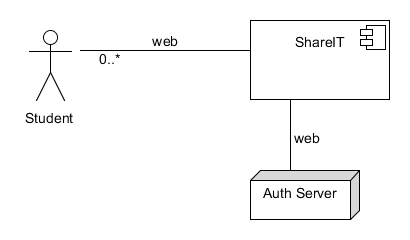
\includegraphics{images/Fachlicher Kontext.png}
\end{center}
\textbf{Student (Benutzer)}

Um mit dem System interagieren zu baut der Student eine Internetverbindung zu diesem auf mit seinem
selbstgewählten Webbrowser und kann nach einer Authentifizierung die Funktionalitäten verwenden.

\textbf{Auth Server (Fremdsystem)}

Das System selber verbindet sich mit einem zuständigen Authentifizierung Server über das Internet oder Intarnet
um sich anmeldende Benutzer zu verifizieren.

\newpage

\subsection{Technischer Kontext}\label{_technischer_kontext}

\begin{center}
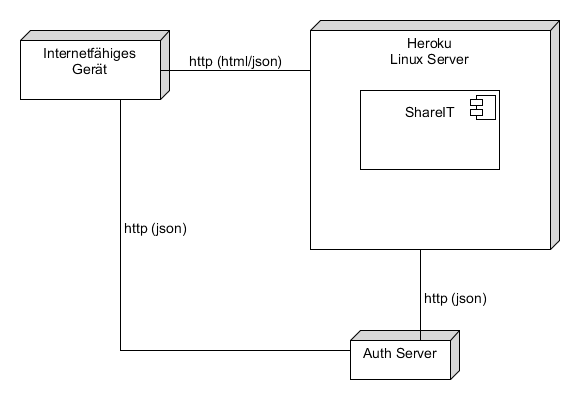
\includegraphics{images/Technischer Kontext.png}
\end{center}

Alle Übertragungen von Informationen erfolgt mit dem ungesicherten Transport Protokoll HTTP

Beim abrufen der Internetpräsenz des Systems wird einmalig das User Interface mit HTML auf das internetfähige Gerät geladen.
Jede weitere Interaktion wird ausschließlich durch das User Interface als JSON Objekt übertragen und empfangen.
Dies betrifft auch die Kommunikation mit dem Fremdsystem.

Für eine detaillierte Auskunft der REST Schnittstellen beider Systeme
die Readmes der Repositoris lesen:

\url{https://github.com/abcshmedu/shareit-summer-2017-ezscheineteam}\\
\url{https://github.com/abcshmedu/a4-auth-server-ezscheineteam}

\section{Lösungsstrategie}\label{section-solution-strategy}
Um eine iterative Entwicklung des Softwaresystems zu ermöglichen und das System auch mittelfristig wartbar und erweiterbar zu erhalten, soll die logische Architektur der Software modular aufgebaut sein. Grundlage dafür ist eine sukzessive Gliederung in fachliche Domänen bzw. Subsysteme  sowie in Schichten.
Zusätzlich wird die Anwendung mit einem REST-API zwischen Web-Browser und Server-Infrastruktur implementiert 

\section{Bausteinsicht}\label{section-building-block-view}

\subsection{Whitebox Gesamtsystem}\label{_whitebox_gesamtsystem}
\begin{center}
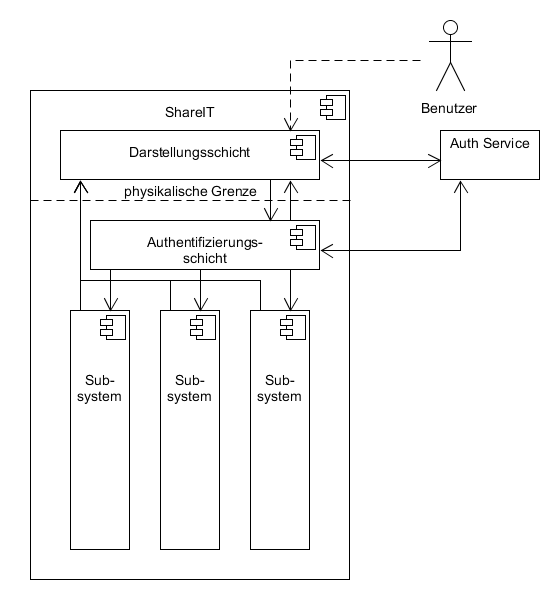
\includegraphics{images/Bausteinsicht E1.png}
\end{center}

\subsubsection{Darstellungsschicht}
 Die Darstellungsschicht (Presentation Layer) kapselt die Benutzungsschnittstelle des Softwaresystems. Sie bildet für den Benutzer den Einstiegspunkt in die Bedienung des Softwaresystems. Ausgehend von den Aktionen des Benutzers auf dieser Benutzungsschnittstelle wie z.B. der Auswahl eines bestimmten Anwendungsfalles werden die dafür erforderlichen Funktionalitäten der API-Schicht angestoßen. Anfallende Ergebnisdaten werden von der API-Schicht an die Darstellungsschicht übergeben, von dieser in geeigneter Form aufbereitet und anschließend dargestellt. Das Softwaresystem ShareIt wird ebenfalls gemäß dieser Konvention als Mehrschichtarchitektur realisiert.

\subsubsection{Authentifizierungsschicht}
Der Authentifizierungsschicht prüft bei jeder eingehenden Anfrage die Authentifizierung des Benutzers und gibt zusätzliche Informationen über diesen an den Subsystemen weiter.
Bei ungültiger Authentifizierung wird eine Fehlermeldung zurückgegeben.

\subsubsection{Subsysteme}
Subsysteme gliedern ein Softwaresystem vertikal nach fachlichen Gesichtspunkten. Dazu werden diejenigen Anwendungsfälle, die thematisch eng miteinander gekoppelt sind (in einer fachlichen Domäne liegen), in ein Subsystem gebündelt. Alternativ wäre es auch denkbar, das Softwaresystem auf der Grundlage des fachlichen Klassenmodells in Subsysteme zu gliedern.

 Die vertikale Gliederung von ShareIt nach thematisch zusammenhängenden Anwendungsfällen ergibt zunächst die folgenden drei fachlichen Domänen:
 \begin{itemize}
\item Benutzerverwaltung 
\item Verwaltung von Medien und Exemplaren 
\item Ausleihe und Rückgabe 
\end{itemize}
\subsection{Ebene 2}\label{_ebene_2}
\begin{center}
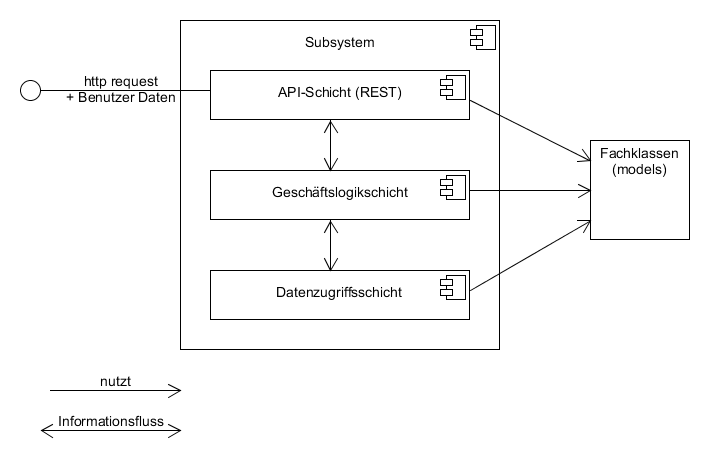
\includegraphics{images/Bausteinsicht E2.png}
\end{center}

\subsubsection{Schichten}
Durch eine Einteilung in Schichten wird das Softwaresystem horizontal gegliedert in verschiedene Abstraktionsebenen. Jede Schicht ist dabei Dienstanbieter für die darüber liegende Schicht und nutzt selbst nur diejenigen Dienste der unmittelbar darunter liegenden Schicht. Die Grenze zwischen den Schichten ist so zu ziehen, dass m¨oglichst wenige Abhängigkeiten über die Schichtgrenzen hinweg bestehen. Ein wesentliches Ziel der Gliederung in Schichten besteht darin, die
Implementierung einer einzelnen Schicht auszutauschen. Die Schnittstellen dieser Schicht bleiben dabei unverändert. Die Abhängigkeiten zwischen den Schichten werden über Schnittstellen gekapselt, sodass die Implementierung jeder einzelnen Schicht austauschbar ist. Modelklassen (Fachklassen) dürfen von allen Schichten, also auch über Schichtengrenzen hinweg, verwendet werden.

\subsubsection{API-Schicht}
Die API-Schicht stellt die Kommunikations-Endpunkte zur Verfügung für Mensch-Maschine (Browser-basiert) und Maschine-Maschine-Interaktionen. Hier werden insbesondere Objekte serialisiert und deserialisiert.

\subsubsection{Geschäftslogikschicht}
Auf der nächsten Abstraktionsebene liegt die Geschäftslogikschicht (Business Layer), die sich auf der Datenzugriffsschicht abstützt. Die Geschäftslogikschicht beinhaltet die grundlegende Geschäftslogik zur Verarbeitung der Fachklassen sowie eine Implementierung der Workflows bzw. Arbeitsabläufe des Systems.

\subsubsection{Datenzugriffsschicht}
Die Datenzugriffsschicht (Persistence Layer) realisiert die Fachklassen sowie den Zugriff auf diejenige Technologie, die zur persistenten Datenhaltung für diese Fachklassen verwendet wird, beispielsweise eine relationale Datenbank. (Die Technologie selbst ist dabei nicht Bestandteil der Datenzugriffsschicht.) Ebenfalls in der Datenzugriffsschicht angesiedelt ist die Abbildung von Objekten auf Strukturen einer Datenbank. Das umfasst beispielsweise das OR-Mapping, also die Abbildung der Objektstruktur der Fachklassen auf relationale Datenbanktabellen, sofern eine relationale Datenbank eingesetzt wird.

\newpage

\section{Verteilungssicht}\label{section-deployment-view}
\begin{center}
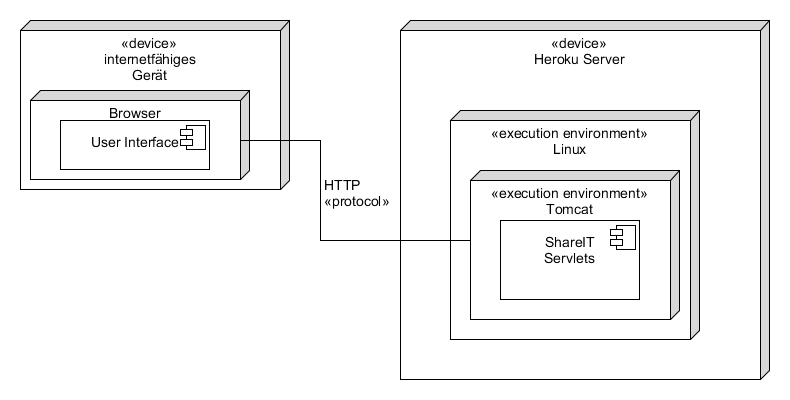
\includegraphics{images/Verteilungssicht.png}
\end{center}
Das User Interface des Systems wird auf dem Gerät des Benutzers innerhalb eines Browsers laufen.
Da diese in JavaScript geschrieben sein soll wird keine Abhängigkeit erzeugt. 
Einzigste Voraussetzung an das Gerät ist eine bestehende Internetverbindung.

Die restlichen Bausteine des Systems werden auf eine Webservice (PaaS) mit dem Namen Heroku (\url{https://www.heroku.com/ }) deployed
um von verschiedenen Orten online abrufbar zu sein.
Für Testzwecke ist ein lokales ausführen auch denkbar.

\newpage

\section{Querschnittliche Konzepte}\label{section-concepts}

\subsection{Persistenz}
Zum dauerhaften speichern von Informationen werden nur die Fachklassen mittels
Nutzung von Hibernate als Object/Relational Mapper auf einer Datenbank gesichert.
Ausschließlich die Datenzugriffsschicht kümmert sich um die Verwaltung der Datenbank.
Als Datenbank verwenden wir HSQL welche im lokalen Ordner db gesichert wird.

\subsection{Logging}
Um eine hilfsreiche Informationsquelle für Entwickler und Administratoren zum Verhalten des Systems zu liefern wird
das Logging Framework log4j verwendet

\subsection{Authentifizierung}
Jeder Benutzer der das System verwenden will muss sich gegenüber diesem sich authentifizieren.
Dafür benötigt der Benutzer ein Token welches er von einem Fremdsystem, den Authentifizierung Server, bei
Angabe von Benutzername und  Passwort erhält. Das Token muss bei jeder Anfrage an das System im HTTP Feld UserToken befinden und gültig sein
da sonst die Anfrage mit einer Fehlermeldung abgewiesen wird. 

\subsection{Fehlermeldungen}
Jede falsche oder ungültige Verwendung des Systems muss mit einer Fehlermeldung als JSON-Objekt beantwortet werden.
Dabei besitzt das JSON-Objekt ein Feld status mit einem HTTP Fehlercode und ein Feld detail mit einer Nachricht die dem 
durchschnittlichen Benutzer den Fehler verständlich mitteilt. Beide Statuscodes von HTTP Response und JSON-Objekt müssen übereinstimmen

\section{Risiken und technische Schulden}\label{section-technical-risks}
\subsection{Datenschutz}
Da bei Informationsaustausch auf das verschlüsselnde Protokoll HTTPS verzichtet wird und stattdessen
das unverschlüsselte Protokoll HTTP verwendet wird können sehr leicht diese Daten von Dritten abgegriffen werden
und sogar dann dazu missbraucht werden sich als eine andere Person gegenüber dem System zu identifizieren. 
\section{Glossar}\label{section-glossary}

\begin{longtable}[]{@{}ll@{}}
\toprule
\begin{minipage}[b]{0.31\columnwidth}\raggedright\strut
Begriff\strut
\end{minipage} & \begin{minipage}[b]{0.63\columnwidth}\raggedright\strut
Definition\strut
\end{minipage}\tabularnewline
\midrule
\endhead
\begin{minipage}[t]{0.31\columnwidth}\raggedright\strut
HTML
\end{minipage} & \begin{minipage}[t]{0.63\columnwidth}\raggedright\strut
Eine textbasierte Auszeichnungssprache zur Strukturierung digitaler Dokumente wie Texte mit Hyperlinks, Bildern und anderen Inhalten.eine textbasierte Auszeichnungssprache zur Strukturierung digitaler Dokumente wie Texte mit Hyperlinks, Bildern und anderen Inhalten.
\end{minipage}\tabularnewline
\begin{minipage}[t]{0.31\columnwidth}\raggedright\strut
HTTP
\end{minipage} & \begin{minipage}[t]{0.63\columnwidth}\raggedright\strut
HyperText Transfer Protocol. Ein zustandsloses Protokoll zur Übertragung von Daten auf der Anwendungsschicht über ein Rechnernetz.
\end{minipage}\tabularnewline
\begin{minipage}[t]{0.31\columnwidth}\raggedright\strut
HTTPS
\end{minipage} & \begin{minipage}[t]{0.63\columnwidth}\raggedright\strut
HyperText Transfer Protocol Secure. Ein Kommunikationsprotokoll im World Wide Web, um Daten abhörsicher zu übertragen.
\end{minipage}\tabularnewline
\begin{minipage}[t]{0.31\columnwidth}\raggedright\strut
JSON
\end{minipage} & \begin{minipage}[t]{0.63\columnwidth}\raggedright\strut
JavaScript Object Notation. Ein kompaktes Datenformat in einer einfach lesbaren Textform zum Zweck des Datenaustauschs zwischen Anwendungen.
\end{minipage}\tabularnewline
\begin{minipage}[t]{0.31\columnwidth}\raggedright\strut
Servlet
\end{minipage} & \begin{minipage}[t]{0.63\columnwidth}\raggedright\strut
Java-Klassen, deren Instanzen innerhalb eines Webservers Anfragen von Clients entgegennehmen und beantworten.
\end{minipage}\tabularnewline
\begin{minipage}[t]{0.31\columnwidth}\raggedright\strut
PaaS
\end{minipage} & \begin{minipage}[t]{0.63\columnwidth}\raggedright\strut
Platform as a Service. Eine Dienstleistung, die in der Cloud eine Computer-Plattform für Entwickler von Webanwendungen zur Verfügung stellt.
\end{minipage}\tabularnewline
\bottomrule
\end{longtable}

\end{document}
